\section{Mengen, Relationen und Funktionen}%
\label{sec:mengen_relationen_und_funktionen}
\subsection{Mengen}%
\label{sub:mengen}

\subsubsection{Schreibweise und Mengenbegriff}%
\label{ssub:schreibweise}
\begin{minipage}{0.9\linewidth}
Zwei Mengen sind genau dann gleich, wenn sie dieselben Elemente enthalten:
$X = Y\, \Leftrightarrow \forall z\, (z \in X \Leftrightarrow z \in Y)$. \\
Sind mathematische Objekte $x_1,\dots,x_n$ gegeben, dann schreiben wir
\[
\{x_1,\dots,x_n\}
\]
für die Menge die als Elemente genau $x_1,\dots,x_n$ hat.
$\{\,\}$: \textit{leere Menge} ($\varnothing$), einzige Menge, die keine Elemente besitzt. 
\end{minipage}

\subsubsection{Teilmengen}%
\label{ssub:teilm}
\begin{minipage}{0.9\linewidth}
$X\subseteq Y$ ($X$ ist eine \textit{Teilmenge} von $Y$), wenn jedes Element von $X$ auch ein Element von $Y$ ist:
\[
X\subseteq Y:\,\Leftrightarrow\,\forall x\,(x\in X\Rightarrow x\in Y).
\]
$X\subsetneq Y$ ($X$ ist eine \textit{echte Teilmenge} von $Y$), falls $X$ eine von $Y$ verschiedene Teilmenge von $Y$ ist:
\[
X\subsetneq Y\,:\Leftrightarrow\, X\subseteq Y\land X\neq Y.
\]
\end{minipage}

\subsubsection{Prädikative Schreibweise}%
\label{ssub:mengeneigenschaft}
\begin{minipage}{0.9\linewidth}
Menge aller Elemente $z$ von $X$ mit der Eigenschaft $\mathsf{E}(z)$.	
\[
\big\{z\in X\mid \mathsf{E}(z)\big\}
\]
oder
\[
\big\{z\mid z\in X\land\mathsf{E}(z)\big\}
\]
\end{minipage}

\subsubsection{Ersetzungsschreibweise}%
\label{ssub:ersetzungsschreibweise}
\begin{minipage}{0.9\linewidth}
\[
\big\{F(x)\mid x\in X \big\}
\]
Menge aller Funktionswerte $F(x)$.
\[
\big\{F(x)\mid x\in X\big\}:=\{y\mid \exists x\in X\,(y=F(x))\}.
\]
\end{minipage}

\subsubsection{Schnittmenge und Vereinigung}%
\label{ssub:schnittmenge_und_vereinigung}
\begin{minipage}{0.9\linewidth}
\[
X\cup Y:=\{x\mid x\in X\lor x\in Y \}
\]
\textit{Vereinigung} von $X$ mit $Y$. \textit{Schnittmenge} von $X$ und $Y$:
\[
X\cap Y:=\{x\in X\mid x\in Y \}=\{x\mid x\in X\land x\in Y\}
\]
Ist $I$ eine Menge so, dass für alle Elemente $i\in I$ auch $A_i$ eine Menge ist, dann wird
\[
\bigcup_{i\in I}A_i:=\{x\mid\exists i\in I\,(x\in A_i) \}.
\]
die Vereinigung von $\{A_i\mid i\in I\}$ genannt.
Analog dazu, ist die \textit{Schnittmenge} durch
\[
\bigcap_{i\in I}A_i:=\{x\mid\forall i\in I\,(x\in A_i) \}
\]
gegeben, falls $I\neq\varnothing$ ist.
\end{minipage}

\subsubsection{Disjunkte Mengen}%
\label{ssub:disjunkte_mengen}
\begin{minipage}{0.9\linewidth}
\textit{disjunkt}: zwei Mengen, die keine gemeinsamen Elemente haben, d.h. \\
$X\cap Y=\varnothing$
\textit{paarweise disjunkt}:
 \[
 \forall i,j\in I\,(i\neq j\Rightarrow A_i\cap A_j=\varnothing).
 \]
\end{minipage}

\subsubsection{Komplementärmenge}%
\label{ssub:komplementärmenge}
\begin{minipage}{0.9\linewidth}
 \[
 X\setminus Y:=\{x\in X\mid x\notin Y\}
 \]
Menge aller Elemente von $X$, die nicht zu $Y$ gehören.
\end{minipage}

\subsubsection{Rechenregeln für Mengen}%
\label{ssub:rechenregeln_für_mengen}
\begin{minipage}{0.9\linewidth}
\begin{enumerate}
 \item Kommutativität der Vereinigung und des Schnittes:
\[
 A\cup B=B\cup A\
 A\cap B=B\cap A.
\]
 \item Assoziativgesetze von Schnitt und Vereinigung:
\[
 A\cap(B\cap C)=(A\cap B)\cap C
 A\cup(B\cup C)=(A\cup B)\cup C
\]
 \item Distributivgesetze von $\cap$ mit $\cup$:
\[
 A\cap(B\cup C)=(A\cap B)\cup (A\cap C)
 A\cup(B\cap C)=(A\cup B)\cap (A\cup C)
\]
 \item Idempotenzgesetz:
\[
  A\cap A=A\
  A\cup A=A
\]
 \item Regeln von DeMorgan:
\[
 (C\backslash A)\cap (C\backslash B)=C\backslash (A\cup B)\\
 (C\backslash A)\cup (C\backslash B)=C\backslash (A\cap B)
\]
 \item Charakterisierung der Teilmengenbeziehung:
\[
 A\subseteq B\Leftrightarrow A\cap B= A\Leftrightarrow A\cup B=B
\]
\end{enumerate}
\end{minipage}

\subsubsection{Potenzmenge}%
\label{ssub:potenzmenge}
\begin{minipage}{0.9\linewidth}
\[
 \mathcal{P}(A):=\{x\mid x\subseteq A\}
\]
\textit{Potenzmenge} von $A$, die genau die Teilmengen von $A$ als Elemente enthält.
\end{minipage}

\subsubsection{Partition}%
\label{ssub:partition}
\begin{minipage}{0.9\linewidth}
\textit{Partition} $P=\{P_i\mid i\in I \}$ = Menge von Teilmengen von $A$, die folgende beiden Voraussetzungen erfüllt:
\begin{itemize}
 \item Die Elemente von $P$ sind nichtleer und paarweise disjunkt.
 \item $\bigcup_{i\in I}P_i=A$
\end{itemize}
Elemente einer Partition = \textit{Blöcke}.
\end{minipage}

\subsection{Relationen, Funktionen und Graphen}%
\label{sub:Relatiinen, Funktionen und Graphen}

\subsubsection{Tupel}%
\label{ssub:tupel}
Ein \textit{n-Tupel} ist ein Term der Form $(x_1,...,x_n)$ wobei $n$ eine natürliche Zahl grösser $0$ ist. \\
Für beliebige Tupel gilt:
\begin{equation}
	(x_1,\dots,x_n)=(y_1,\dots,y_k):\Leftrightarrow n=k\land x_1=y_1\land\dots\land y_n=x_n.
\end{equation}
2-Tupel nennen wir \textit{Paare} und 3-Tupel \textit{Tripel}.

\subsubsection{Kartesisches Produkt}%
\label{ssub:kartesisches_produkt}
\begin{minipage}{0.9\linewidth}
\begin{align*}
\prod_{i=1}^{n}A_i=\big\{(a_1,\dots,a_n)\mid a_1\in A_1\land\dots\land a_n\in A_n \big\}.
\end{align*}
Das \textit{kartesische} Produkt von $A_1, ..., A_n$ ist die Menge aller $n$-Tupel mit Einträgen aus den Mengen $A_1,
..., A_n$ 
\\
Für das kartesische Produkt von zwei Mengen schreibt man:
\[
X\times Y:=\{(x,y)\mid x\in X\land y\in Y \}.
\]
\end{minipage}

\subsubsection{Relationen}%
\label{ssub:relationen}
\begin{minipage}{0.9\linewidth}
Eine $n$-Stellige \textit{Relation R} ist eine Menge von $n$-Tupeln aus $A_1 \times \dots \times A_n$.
\begin{align*}
R\subseteq A_1\times\dots \times A_n.
\end{align*}
Ist $R$ eine $n$-stellige Relation und gilt $(x_1,\dots,x_n)\in R$, dann sagen wir, dass die Elemente $x_1,\dots,x_n$ zueinander in Relation $R$ stehen.
Eine $2$-stellige Relation $R\subseteq X\times Y$ heisst auch eine \textit{binäre Relation} auf den Mengen $X$ und $Y$. Ist $R$ eine binäre Relation, so schreiben wir auch $xRy$ für $(x,y)\in R$.
\end{minipage}

\subsubsection{Graphen}%
\label{ssub:graphen}
\begin{minipage}{0.9\linewidth}
Ein \textit{(gerichteter) Graph} ist ein Paar $G=(V,E)$ bestehend aus einer Menge $V$ (Knotenmenge) und einer binären Relation $E\subseteq V\times V$ (Kantenmenge).
\end{minipage}

\subsubsection{Funktionen}%
\label{ssub:funktionen}
\begin{minipage}{0.9\linewidth}
Eine Relation $f\subseteq A \times B$ ist eine \textit{Funktion} von $A$ nach $B$, falls:
\begin{align*}
\forall x\in A\exists!y\in B((x,y)\in f)
\end{align*}
gilt. In diesem Fall schreiben wir
\begin{align*}
f:A\to B.
\end{align*}
\end{minipage}

\begin{minipage}{0.9\linewidth}
Im Kontext einer Funktion $f:A\to B$ verwenden wir folgende Schreibweisen und Konventionen:
\begin{itemize}
 \item Da zu jedem $x\in A$ ein eindeutig bestimmtes Element $y\in B$ mit $(x,y)\in f$ existiert, kann dieses $y$ mit $f(x)$ bezeichnet und \textit{Funktionswert von $f$ bei $x$} genannt werden.
 \item Die Menge aller Funktionswerte $Im(f) := \{f(x)\mid x\in A \}$ wird als \textit{Bild(menge)} von $f$ bezeichnet.
 \item Die Menge $A$ nennen wir den Definitionsbereich von $f$ und schreiben dafür auch $Dom(f)$.
 \item Der Definitionsbereich ist eindeutig durch die Funktion gegeben:
  \begin{align*}
   A=Dom(f)=\{x\mid \exists y ((x,y)\in f) \}=\{x\mid \exists y (f(x)=y )\}
  \end{align*}
 \item Die Menge $B$ ist durch die Voraussetzung $f:A\to B$ nicht eindeutig bestimmt, tatsächlich gilt $f:A\to B$ für jede Menge $B$ mit $Im(f)\subseteq B$.
\end{itemize}	
\end{minipage}

\subsubsection{Funktionen - Komposition}%
\label{ssub:funktionen_koposition}
\begin{minipage}{0.9\linewidth}
\begin{align*}
 &g\circ f:A\to C\\
 (&g\circ f)(x)=g(f(x))
\end{align*}
\end{minipage}

\begin{minipage}[t]{0.45\linewidth}
\subsubsection{Injektive Funktion}%
\label{ssub:injektive_funktion}
Eine Funktion $f$ ist genau dann \textit{injektiv}, wenn die Relation
    \begin{align*}
        f^{-1}=\{(y,x)\mid (x,y)\in f\}
    \end{align*}
    eine Funktion ist. Ist $f:A\to B$ eine injektive Funktion, dann nennt man $f^{-1}:Im(f)\to A$ die \textit{Umkehrfunktion} oder \textit{inverse Funktion} von $f$.
\end{minipage}
\hfill
\begin{minipage}[t]{0.45\linewidth}
\subsubsection{Surjektive Funktion}%
\label{ssub:injektive_funktion}
Eine Funktion $f:A\to B$ heisst \textit{surjektiv} auf $B$, wenn $B=Im(f)$. Ist die Funktion $f$ zusätzlich injektiv, so sagen wir $f:A\to B$ sei \textit{bijektiv}.	
\end{minipage}

\subsubsection{Beispiel - Injektiv Surjektiv}%
\label{ssub:beispiel_injektiv_surjektiv}
\begin{minipage}{0.9\linewidth}
   \begin{center}
        %\centering
    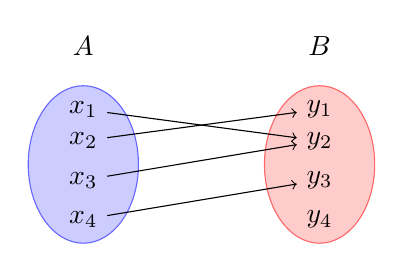
\begin{tikzpicture}
        % draw the sets
        \filldraw[fill=blue!20, draw=blue!60] (-1.5,0) circle [x radius=0.7cm, y radius=1cm];
        \filldraw[fill=red!20, draw=red!60] (1.5,0) circle [x radius=0.7cm, y radius=1cm];


        % the texts
        \node at (-1.5,1.5) {$A$};
        \node at (1.5,1.5) {$B$};

        % the points in the sets (here I just create nodes to use them later on to position
        % the circles and the arrows
        \node (x1) at (-1.5,0.7) {$x_1$};
        \node (x2) at (-1.5,0.3) {$x_2$};
        \node (x3) at (-1.5,-0.2) {$x_3$};
        \node (x4) at (-1.5,-0.7) {$x_4$};
        \node (y1) at (1.5,0.7) {$y_1$};
        \node (y2) at (1.5,0.3) {$y_2$};
        \node (y3) at (1.5,-0.2) {$y_3$};
        \node (y4) at (1.5,-0.7) {$y_4$};

        % draw the arrows
        \draw[->] (x1) -- (y2);
        \draw[->] (x2) -- (y1);
        \draw[->] (x3) -- (y2);
        \draw[->] (x4) -- (y3);

    \end{tikzpicture}
    \end{center}
    \begin{itemize}
        \item Die Funktion ist wegen $f(x_1)=f(x_3)$ nicht injektiv.
        \item Die Funktion ist wegen $y_4\in B$ nicht surjektiv auf $B$.
        \item Die Funktion ist surjektiv auf $\{y_1,y_2,y_3\}$.
    \end{itemize}	
\end{minipage}

\subsubsection{Endliche und unendliche Mengen}%
\label{ssub:endliche_und_unendliche_mengen}
\begin{itemize}
\item Eine Menge $X$ heisst \textit{endlich}, wenn es eine natürliche Zahl $n$ und eine Darstellung der Form $X=\{x_1,x_2,\dots,x_n\}$ gibt. Wenn $X=\{x_1,\dots,x_n\}$ gilt, und die Elemente $x_i$ paarweise verschieden sind (d.h. es gilt $i\neq j\Rightarrow x_i\neq x_j$), dann hat die Menge $X$ genau $n$ viele Elemente und wir schreiben $|X|=n$.
\item Nicht endliche Mengen nennen wir \textit{unendlich}.
\item Eine Menge $X$ heisst \textit{abzählbar}, wenn eine surjektive Funktion $F:\to X$ existiert oder wenn $X=\varnothing$ gilt.
\item Die Menge $X$ heisst \textit{abzählbar unendlich}, wenn $X$ abzählbar und unendlich ist.
\item Eine \textit{überabzählbare} Menge ist eine Menge, die nicht abzählbar ist.
\end{itemize}

\begin{minipage}{0.9\linewidth}
\subsubsection{Lemma 1}%
\label{ssub:lemma_1}
Wenn $n$ Objekte auf $m$ Behälter verteilt werden und $n>m$ gilt, dann gibt es mindestens einen Behälter, der mehr als ein Objekt enthält. Formal, sind $n>m$ natürliche Zahlen und gelte $|X|= n$ sowie $|Y|=m$, dann gibt es keine injektive Funktion
\begin{align*}
 F: X\to Y.
\end{align*}
\end{minipage}

\begin{minipage}{0.9\linewidth}
\subsubsection{Lemma 2}%
\label{ssub:lemma_2}
Gibt es eine injektive Funktion $F:\mathbb{N}\to A$, dann ist die Menge $A$ unendlich.
    Es sei eine Menge $A$ und eine injektive Funktion $F:\mathbb{N}\to A$ gegeben. Wäre die Menge $A$ endlich, dann gäbe es eine natürliche Zahl $n$ mit $|A|=n$. Die Funktion
    \begin{align*}
    G&:\{0,\dots,n\}\to A\\
    G&(x) = F(x)
    \end{align*}
    wäre injektiv und würde, wegen $|\{0,\dots,n\}|=n+1$, dem Schubfachprinzip widersprechen.
\end{minipage}

\subsubsection{Sätze zu Mengen}%
\label{ssub:sätze_zu_mengen}
\textbf{Satz } 	
    Folgende Aussagen sind für unendliche Mengen $A$ äquivalent:
    \begin{enumerate}
        \item Die Menge $A$ ist abzählbar.
        \item Es gibt eine surjektive Funktion $F_{\mathbb{N},A}:\mathbb{N}\to A$.
        \item Es gibt eine injektive Funktion $F_{A,\mathbb{N}}:A\to\mathbb{N}$.
        \item Es gibt eine bijektive Funktion $B_{\mathbb{N},A}:\mathbb{N}\to A$.
        \item Es gibt eine bijektive Funktion $B_{A,\mathbb{N}}:A\to\mathbb{N}$.
    \end{enumerate}
   \textit{\textbf{Beweis: }} 
 \begin{itemize}
        \item Die Aussagen in $a)$ und $b)$ sind per Definition äquivalent.
        \item Die Aussagen in $d)$ und $e)$ sind offensichtlich äquivalent (Umkehrfunktion).
        \item Für die Implikation $b)\Rightarrow c)$ definieren wir
        \begin{align*}
            F_{A,\mathbb{N}}(a)=\min\{n\in\mathbb{N} \mid F_{\mathbb{N},A}(n)=a\},
        \end{align*}
        dies ist gerechtfertigt, da aus der Surjektivität von $F_{\mathbb{N},A}:\mathbb{N}\to A$ folgt, dass zu jedem $a\in A$ mindestens ein $n\in\mathbb{N}$ mit $F_{\mathbb{N},A}(n)=a$ existiert. Es bleibt die Injektivität von $F_{A,\mathbb{N}}$ nachzuweisen, dazu nehmen wir $F_{A,\mathbb{N}}(a)=F_{A,\mathbb{N}}(a')$ an. Es folgt, dass es eine natürliche Zahl $n$ mit $F_{\mathbb{N},A}(n)=a$ und $F_{\mathbb{N},A}(n)=a'$ gibt. Somit muss wie gewünscht $a=a'$ gelten.
        \item Für die Implikation $c)\Rightarrow b)$, gehen wir von einer injektiven Funktion $F_{A,\mathbb{N}}:A\to\mathbb{N}$ aus.
        Weil diese Funktion injektiv ist, und weil $Dom(F_{A,\mathbb{N}})=A$ gilt, ist
        \begin{align*}
            F_{A,\mathbb{N}}^{-1}:Im(F_{A,\mathbb{N}}) \to A
        \end{align*}
        eine surjektive Funktion. Um eine surjektive Funktion von $\mathbb{N}$ nach $A$ zu erhalten, brauchen wir bloss noch die ``restlichen'' Elemente aus $\mathbb{N}$ zuzuordnen, dazu wählen wir ein beliebiges Element aus $a\in A$ und setzen:
        \begin{align*}
            F_{\mathbb{N},A}(n)=
                \begin{cases}
		F_{A,\mathbb{N}}^{-1}(n)&\text{falls }n\in Im(F_{A,\mathbb{N}})\\
                a&\text{sonst}
                \end{cases}
        \end{align*}
        \item Wenn wir die Implikation $b)\Rightarrow d)$ zeigen, dann ist alles bewiesen. Wir müssen, ausgehend von einer unendlichen Menge $A$ und einer surjektiven Abbildung $F_{\mathbb{N},A}: \mathbb{N}\to A$, eine bijektive Abbildung $B_{\mathbb{N},A}: \mathbb{N}\to A$ konstruieren. Da uns für einen vollständigen Beweis die Werkzeuge noch fehlen (Rekursion), wollen wir hier bloss eine Beweisskizze präsentieren. Wir definieren die Funktion $B_{\mathbb{N},A}$ rekursiv wie folgt:
        \begin{align*}
        B_{\mathbb{N},A}(0) &= F_{\mathbb{N},A}(0)\\
        B_{\mathbb{N},A}(n+1) &= F_{\mathbb{N},A}(\min\{k\in\mathbb{N}\mid F(k)\neq B_{\mathbb{N},A}(0),\dots,B_{\mathbb{N},A}(n) \})
        \end{align*}
        Die resultierende Funktion ist auf ganz $\mathbb{N}$ definiert, weil die Menge $A$ unendlich ist (würde die Rekursion abbrechen, dann wäre $A$ von der Form $\{F_{\mathbb{N},A}(0),\dots,F_{\mathbb{N},A}(m)\}$ für ein $m\in\mathbb{N}$). Die Funktion $B_{\mathbb{N},A}$ ist surjektiv, weil $F_{\mathbb{N},A}$ surjektiv ist. Die Injektivität folgt, weil per Konstruktion für alle $x,y$
        \begin{align*}
        x<y \Rightarrow B_{\mathbb{N},A}(x) \neq B_{\mathbb{N},A}(y)
        \end{align*}
        gilt.\qedhere
    \end{itemize}
\textbf{Satz } Jede endliche Menge ist abzählbar. \\
\textit{\textbf{Beweis: }}
Ist $X$ eine endliche Menge, dann können wir $X$ als $\{x_1,\dots,x_n\}$ mit einer natürlichen Zahl $n$ schreiben. Da die leere Menge per Definition abzählbar ist, können wir annehmen, dass $X$ mindestens ein Element $x_1$ besitzt. Wir definieren nun die Funktion $F:\mathbb{N}\to X$ mit
\begin{align*}
F(i)=\begin{cases}
x_i&\text{falls }0<i\leq n\\
x_1&\text{sonst.}
\end{cases}
\end{align*}
Da $F$ offensichtlich jedes Element von $X=\{x_1\dots x_n\}$ trifft, ist $F$ surjektiv. Somit ist $X$ abzählbar. \\

\textbf{Satz } Jede Teilmenge einer abzählbaren Menge ist abzählbar.\\
\textit{\textbf{Beweis: }}
Es sei $X\subseteq Y$ und $Y$ sei eine abzählbare Menge. Da $Y$ abzählbar ist,
gibt es eine surjektive Funktion $F:\mathbb{N}\to Y$. Wenn $X=\varnothing$ gilt, dann
ist $X$ per Definition abzählbar und wir sind fertig. Ist $X\neq\varnothing$,
dann gibt es ein Element $a\in X$. Wir können nun wie folgt eine Abbildung
$G:\mathbb{N}\to X$ angeben.
\begin{align*}
G(x)=\begin{cases}
F(x)&\text{falls }F(x)\in X\\
a&\text{sonst.}
\end{cases}
\end{align*}
Da $X\subseteq Y$ gilt und weil jedes Element von $Y$ von der Funktion $F$
getroffen wird, wird auch jedes Element von $X$ von $G$ getroffen. Somit
ist $G:\mathbb{N}\to X$ surjektiv und $X$ ist also abzählbar. \\

\textbf{Satz } Ist $X$ eine abzählbare Menge und gibt es eine surjektive Funktion $F:X\to Y$, dann ist auch $Y$ abzählbar. \\
\textit{\textbf{Beweis: }} 
Sollte $X$ die leere Menge sein, dann ist auch $Y$ leer und somit abzählbar. Ist $X$ nichtleer, dann folgt aus der Abzählbarkeit von $X$, dass es eine surjektive Abbildung $G:\mathbb{N}\to X$ gibt. Wir können nun die Funktion $H:\mathbb{N}\to Y$ durch Komposition der Funktionen $F$ und $G$ bilden, d.h. wir definieren
\begin{align*}
H:\mathbb{N}\to Y\phantom{abstand}\text{ mit }\phantom{abstand} H(n)=F(G(n)).
\end{align*}
Wir müssen nun noch zeigen, dass wir mit der Funktion $H$ jedes Element von $Y$ treffen. Wir nehmen dazu ein beliebiges Element $y$ von $Y$ und zeigen, dass es eine natürliche Zahl $n$ gibt mit $H(n)=y$. Es sei also $y\in Y$ beliebig. Da die Funktion $F:X\to Y$ surjektiv ist, muss es ein $x\in X$ geben so, dass $F(x)=y$ gilt. Weil aber auch die Funktion $G:\mathbb{N}\to X$ surjektiv ist, muss es ebenfalls eine natürliche Zahl $n$ geben, mit $G(n)=x$. Zusammenfassend können wir also sagen, dass es eine natürliche Zahl und ein Element $x$ aus $X$ gibt, mit der Eigenschaft
\[
H(n)=F(G(n))=F(x)=y.
\]
Weil $y\in Y$ beliebig gewählt wurde, ist die Funktion $H$ surjektiv. \\

\textbf{Satz} (Erstes Diagonalargument) 
Die Menge $\mathbb{N}\times\mathbb{N}$, bestehend aus allen Paaren von natürlichen Zahlen, ist abzählbar.\\
\textit{\textbf{Beweis: }} 
Anstelle eines formalen Beweises, skizzieren wir eine Abzählung aller Paare von natürlichen Zahlen wie folgt:
%\begin{figure}[h!]
\begin{center}
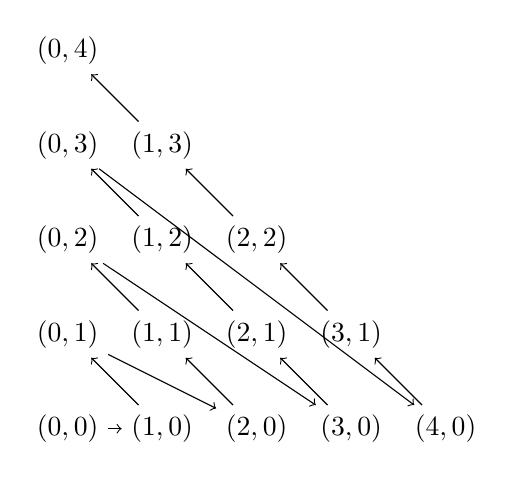
\begin{tikzpicture}[scale=1.2]
\node (0) at (0,0) {$(0,0)$};
\node (2) at (0,1) {$(0,1)$};
\node (5) at (0,2) {$(0,2)$};
\node (9) at (0,3) {$(0,3)$};
\node (14) at (0,4) {$(0,4)$};
\node (1) at (1,0) {$(1,0)$};
\node (4) at (1,1) {$(1,1)$};
\node (8) at (1,2) {$(1,2)$};
\node (13) at (1,3) {$(1,3)$};
\node (3) at (2,0) {$(2,0)$};
\node (7) at (2,1) {$(2,1)$};
\node (12) at (2,2) {$(2,2)$};
\node (6) at (3,0) {$(3,0)$};
\node (11) at (3,1) {$(3,1)$};
\node (10) at (4,0) {$(4,0)$};
\draw[->] (0) -- (1);
\draw[->] (1) -- (2);
\draw[->] (2) -- (3);
\draw[->] (3) -- (4);
\draw[->] (4) -- (5);
\draw[->] (5) -- (6);
\draw[->] (6) -- (7);
\draw[->] (7) -- (8);
\draw[->] (8) -- (9);
\draw[->] (9) -- (10);
\draw[->] (10) -- (11);
\draw[->] (11) -- (12);
\draw[->] (12) -- (13);
\draw[->] (13) -- (14);
\end{tikzpicture}
%\includegraphics[width=0.3\textwidth]{figures/cantor1}
%\caption*{Die Pfeile deuten die Reihenfolge an, in der die Elemente von $\mathbb{N}\times\mathbb{N}$ abgezählt werden.}
\end{center}
\ %end{figure}

\textbf{Satz }
Jede Vereinigung von abzählbar vielen abzählbaren Mengen ist abzählbar. Konkret, jede Vereinigung von der Form
\[
\bigcup_{i\in\mathbb{N}}A_i
\]
ist abzählbar, wenn alle $A_i$'s abzählbar sind.
\textbf{\textit{Beweis: }}
Wir nehmen an, dass die Menge $\{A_i\mid i\in \mathbb{N} \}$ aus lauter abzählbaren Mengen besteht. Um zu zeigen, dass $\bigcup_{i\in N}A_i$ abzählbar ist, genügt es, aufgrund von Satz~\ref{satz:abzaehlbarTransitiv} und Satz~\ref{cantor1}, zu zeigen, dass es eine surjektive Funktion
\[
H:\mathbb{N}\times\mathbb{N}\to\bigcup_{i\in N}A_i
\]
gibt. Da für jede natürliche Zahl $i$ die Menge $A_i$ abzählbar ist, gibt es für jede natürliche Zahl $i$ auch eine surjektive Funktion $F_i:\mathbb{N}\to A_i$. Wir können die Vereinigungsmenge der $A_i$'s also wie folgt schreiben:
\begin{align*}
\bigcup_{i\in \mathbb{N}}A_i&=\{F_i(j)\mid i,j\in\mathbb{N} \}\\
&=\{F_i(j)\mid (i,j)\in\mathbb{N}\times\mathbb{N} \}.
\end{align*}
Daraus folgt, dass die Funktion
\[
H:\mathbb{N}\times\mathbb{N}\to \bigcup_{i\in N}A_i\phantom{abstand}\text{mit}\phantom{abstand} H(i,j)=F_i(j),
\]
die gesuchte surjektive Funktion ist. \\
\textbf{Folgerung }
Die Menge $\mathbb{Z}\times \mathbb{Z}$ ist abzählbar.
\textbf{\textit{Beweis: }}
\begin{align*}
X&=\mathbb{N}\times\{-n\mid n\in \mathbb{N}\}\\
Y&=\{-n\mid n\in \mathbb{N}\}\times\mathbb{N} \\
Z&=\{-n\mid n\in \mathbb{N}\}\times\{-n\mid n\in \mathbb{N}\}
\end{align*}
abzählbar sind. Aus Satz~\ref{satz:countableUnion} folgt also, dass die Menge
\[
\mathbb{Z}\times\mathbb{Z}=(\mathbb{N}\times\mathbb{N})\cup X\cup Y\cup Z
\]
abzählbar ist. \\
\textbf{Folgerung }
Die Menge $\mathbb{Q}=\big\{\frac{x}{y}\mid x,y\in \mathbb{Z}\big\}$ der rationalen Zahlen (Brüche) ist abzählbar.
\textbf{\textit{Beweis: }}
Da die Funktion
\[
F:\mathbb{Z}\times(\mathbb{Z}\setminus{\{0\}})\to \mathbb{Q}\phantom{abstand}\text{mit}\phantom{abstand}F(x,y)=\frac{x}{y}
\]
surjektiv ist, folgt die Behauptung aus Satz~\ref{satz:abzaehlbarTransitiv}.\\

\subsubsection{Theorem 2}%
\label{ssub:theorem_2}
Die Menge aller unendlichen Binärsequenzen (Sequenzen aus Nullen und Einsen) ist überabzählbar.
\textbf{\textit{Beweis: }}
Beweis durch Widerspruch. Wäre die Menge aller unendlichen Binärsequenzen abzählbar, dann gäbe es eine Liste von der Form\footnote{Natürlich ist die angedeutete Liste Beispielhaft und dient nur der Veranschaulichung unserer Konstruktion der Sequenz $b$. Die Sequenz $s_0$, beispielsweise, könnte auch mit dem Präfix $00000100$ oder irgend einer anderen Folge von Nullen und Einsen beginnen. }
\begin{center}
\begin{tabular}{c|l}
$\mathbb{N}$ & Binärsequenzen\\
\hline
$0$ & $s_0=01101011\cdots$\\
$1$ & $s_1=10010110\cdots$\\
$2$ & $s_2=00101001\cdots$\\
$\vdots$ & $\vdots$
\end{tabular}
\end{center}
in der alle unendlichen Binärsequenzen vorkommen. Wir konstruieren nun, ausgehend von dieser Liste, eine Binärsequenz $b$, die nicht in der Liste enthalten sein kann. Wir definieren $b$ wie folgt:
\begin{align*}
0\text{-tes Glied}&=b(0)=1-s_0(0)\\
1\text{-tes Glied}&=b(1)=1-s_1(1)\\
2\text{-tes Glied}&=b(2)=1-s_2(2)\\
&\vdots\\
n\text{-tes Glied}&=b(n)=1-s_n(n)\\
&\vdots
\end{align*}
Die Folge $b=110\cdots$ kann nicht in der Liste vorkommen, weil sie sich von jedem Element in der Liste in mindestens
einem Glied unterscheidet (von der $n$-ten Sequenz unterscheidet sich $b$ im $n$-ten Glied). Dies steht im Widerspruch
zu unserer Annahme, dass in der Liste alle unendlichen Binärsequenzen vorkommen.\\
\textbf{Folgerung }
Das Intervall $(0,1)=\{r\in\mathbb{R}\mid 0<r<1 \}$ ist überabzählbar. Insbesondere ist die Menge $\mathbb{R}$ der reellen Zahlen
überabzählbar.\\
\textbf{\textit{Beweis: }}
Die reellen Zahlen (in Binärdarstellung) im Intervall $(0,1)$, sind von der Form $0,\dots$ wobei $\dots$ für eine
unendliche Binärsequenz steht. Daher steht das Intervall $(0,1)$ mit der Menge aller unendlichen Binärsequenzen in
eins-zu-eins Korrespondenz. Die Behauptung folgt daher aus Theorem~\ref{thrm:cantor2}.\\
\textbf{Folgerung }
Die Potenzmenge von $\mathbb{N}$ ist überabzählbar. \\
\textbf{\textit{Beweis: }}
Jede Teilmenge $A$ von $\mathbb{N}$ kann wie folgt durch eine Binärsequenz $\chi_A$ beschrieben werden:
\begin{align*}
\chi_A(n)=\begin{cases}
1&\text{falls } n\in A\\
0&\text{falls} n\notin A.
\end{cases}
\end{align*}
Daher folgt die Behauptung aus Theorem~\ref{thrm:cantor2}.\\
\textbf{Folgerung }
Die Menge aller Funktionen $F:\mathbb{N}\to\mathbb{N}$ ist überabzählbar. \\
\textbf{\textit{Beweis: }}
Die Menge der Binärsequenzen entspricht der Menge der Funktionen $F:\mathbb{N}\to\{0,1\}$. Daher folgt die Behauptung
aus Theorem~\ref{thrm:cantor2}. \\
\textbf{Folgerung }
Es gibt Funktionen $F:\mathbb{N}\to\mathbb{N}$, die von keinem Java, C, C++, Fortran\dots Programm berechenbar sind. Solche Funktionen heissen \textit{unberechenbar}.

\subsection{Ordnungs- und Äquivalenzrelationen}%
\label{sub:ordnungs_und_äquivalenzrelationen}

\subsubsection{Binäre Relationen}%
\label{ssub:binäre_relationen}
Eine binäre Relation $R$ auf einer Menge $X$ heisst:
    \begin{itemize}
    \item \textit{Reflexiv}, wenn für alle $x\in X$
    \[
    xRx
    \]
    gilt.
    \item \textit{Symmetrisch}, wenn für alle $x,y\in X$
    \[
    xRy\,\Rightarrow\, yRx
    \]
    gilt.
    \item \textit{Antisymmetrisch}, wenn für alle $x,y\in X$
    \[
xRy\land yRx\,\Rightarrow x=y
\]
gilt.
\item \textit{Transitiv}, wenn für alle $x,y,z\in X$
\[
xRy\land yRz\,\Rightarrow \, xRz
\]
gilt.
\end{itemize}
\subsubsection{Äquivalenzrelationen}%
\label{ssub:äquivalenzrelationen}
\textit{Äquivalenzrelationen} sind reflexive, symmterische und transitive Relationen.

\subsubsection{Äquivalenzklassen}%
\label{ssub:äquivalenzklassen}
Es sei $R$ eine Äquivalenzrelation auf einer Menge $X$ und $x\in X$. Die \textit{Äquivalenzklasse} $[x]_R$ von $x$ bezüglich $R$ ist die Menge aller Elemente von $X$, die zu $x$ in Relation $R$ stehen:
    \[
    [x]_R:=\{y\in X\mid xRy \}
    \]
    Jedes Element einer Äquivalenzklasse nennen wir einen \textit{Repräsentanten} der entsprechenden Äquivalenzklasse.
    Die \textit{Faktormenge} $X/R$ \textit{von} $X$ \textit{modulo} $R$ ist die Menge aller Äquivalenzklassen:
    \[
    X/R:=\big\{ [x]_R\mid x\in X \big\}
    \]

\subsubsection{Lemma 3}%
\label{ssub:lemma_3}
Ist $\sim $ eine Äquivalenzrelation auf einer Menge $X$ und gilt $x,y\in X$ mit $x\sim y$, dann gilt $[x]_\sim=[y]_\sim$. Mit anderen Worten, äquivalente Elemente repräsentieren stets dieselbe Äquivalenzklasse.
\textbf{\textit{Beweis: }} 
Seien $X,\sim,x,y$ wie in der Behauptung. Um zu zeigen, dass $[x]_\sim=[y]_\sim$ gilt, genügt es nachzuweisen, dass $x\sim z\Leftrightarrow y\sim z$ für beliebige $z\in X$ gilt. Wir nehmen $x\sim y$ an, dann gilt
    \begin{align*}
    y\sim z\Rightarrow x\sim y\land y\sim z \stackrel{\text{Transitivität}}{\Longrightarrow} x\sim z
    \end{align*}
    und
    \[
    x\sim z\Rightarrow x\sim y\land x\sim z\stackrel{\text{Symmetrie}}{\Longrightarrow} y\sim x\land x\sim z\stackrel{\text{Transitivität}}{\Longrightarrow} y\sim z,
    \]
    wie gewünscht. \\
\textbf{Folgerung: } 
Ist $\sim $ eine Äquivalenzrelation auf $X$ und sind $x,y\in X$ mit $x\in[y]_\sim$, dann gilt $[x]_\sim=[y]_\sim$. Mit anderen Worten, jedes Element einer Äquivalenzklasse ist auch ein Repräsentant dieser Äquivalenzklasse.
\textbf{\textit{Beweis: }}
Es seien $X,\sim,x$ und $y$ wie in der Behauptung. Aus $x\in[y]_\sim$ folgt $y\sim x$. Die Behauptung folgt nun aus Lemma~\ref{lm:sim gleiche klasse}.

\subsubsection{Sätze zu Äquivalenzrelationen}%
\label{ssub:sätze_zu_äquivalenzrelationen}
\textbf{Satz }
  Ist $\sim $ eine Äquivalenzrelation auf $X$ und sind $x,y\in X$ mit $[x]_\sim\neq[y]_\sim$, dann gilt $[x]_\sim\cap[y]_\sim=\varnothing$.
    Mit anderen Worten, verschiedene Äquivalenzklassen sind immer disjunkt.\\
\textbf{\textit{Beweis: }} 
Es seien $X,\sim,x$ und $y$ wie in der Behauptung. Wir zeigen die Kontraposition, d.h.
    \[
    [x]_\sim\cap[y]_\sim\neq\varnothing\Rightarrow [x]_\sim=[y]_\sim.
    \]
    Es gelte also $[x]_\sim\cap[y]_\sim\neq\varnothing$, es gibt daher ein $z\in [x]_\sim\cap[y]_\sim$. Daraus folgt,
    dass $x\sim z\land y\sim z$ gilt und wegen der Transitivität und der Symmetrie von $\sim$ folgt sofort $x\sim y$.
    Die Behauptung folgt nun aus Lemma.\\
\textbf{Satz }
Ist $\sim$ eine Äquivalenzrelation auf einer Menge $X$, dann ist die Faktormenge $X/\sim$ eine Partition von $X$.\\ 
\textbf{\textit{Beweis: }} 
Es sei $\sim$ eine beliebige Äquivalenzrelation auf einer Menge $X$. Wir müssen folgende Punkte verifizieren:
    \begin{enumerate}
    \item\label{a} Die Äquivalenzklassen sind alle nichtleer.
    \item\label{2} Die Äquivalenzklassen paarweise disjunkt.
    \item\label{3} Es gilt
    \[
    \bigcup_{x\in X}[x]_{\sim}=X.
    \]
    \end{enumerate}
    Der erste Punkt folgt aus der Definition von der Faktormenge (die Äquivalenzklassen sind via ihrer Repräsentanten definiert). Die Tatsache, dass die Äquivalenzklassen paarweise disjunkt sind, ist genau die Aussage von Satz~\ref{satz: equivalenzklassen disjunkt}. Wir brauchen also bloss noch den letzten Punkt zu verifizieren. Dies folgt, da für jedes $z\in X$, wegen der Transitivität von $\sim$, $z\sim z$ und somit
    \[
    z\in[z]_\sim\subseteq\bigcup_{x\in X}[x]_\sim
    \]
    gilt.\\
\textbf{Satz }
    Ist $P=\{A_i\mid i\in I\}$ eine Partition von der Menge $X$, dann ist die Relation $\sim$, gegeben durch
    \[
    x\sim y:\Leftrightarrow \exists i\in I\,(x\in A_i\land y\in A_i),
    \]
    eine Äquivalenzrelation auf $X$. Zusätzlich gilt
    \[
    X/\sim=P.
    \]\\
\textbf{\textit{Beweis: }} 
Zuerst zeigen wir, dass die Relation $\sim$ unter den gegebenen Umständen eine Äquivalenzrelation ist.
    \begin{itemize}
    \item \textbf{Reflexivität}: Sei $x\in X$  beliebig. Wir müssen zeigen, dass $x\sim x$ gilt. Da $P=\{A_i\mid i\in I\}$ eine Partition von $X$ ist, gibt es ein $i\in I$ mit $x\in A_i$, daraus folgt sofort $x\sim x$.
    \item \textbf{Symmetrie}: Es gelte $x\sim y$. Wir müssen $y\sim x$ zeigen. Aus $x\sim y$ folgt, dass es ein $i\in I$ mit $x\in A_i\land y\in A_i$ gibt, dies ist offensichtlich äquivalent zu $y\sim x$.
    \item \textbf{Transitivität}: Es gelte $x\sim y\land y\sim z$. Wir müssen $x\sim z$ zeigen. Aus $x\sim y\land y\sim z$ folgt, dass es $i,j\in I$ gibt so, dass $x,y\in A_i$ und $y,z\in A_j$ gilt. Da $P=\{A_i\mid i\in I\}$ eine Partition ist, kann $y $ nicht in zwei verschiedenen Blöcken enthalten sein, es gilt daher $i=j$ und somit $x\sim z$.
    \end{itemize}
    Dass die Äquivalenzklassen von $\sim$ genau den Blöcken von $P$ entsprechen ist sofort klar, wenn man beachtet, dass
    zwei Elemente genau dann äquivalent sind, wenn sie im selben Block von $P$ liegen.\\
\textbf{Satz }
Für jede Relation $\sim$ auf einer Menge $X$ sind folgende beiden Aussagen äquivalent.
    \begin{enumerate}
    \item[1.] Die Relation $\sim$ ist eine Äquivalenzrelation.
    \item[2.] Es gibt eine Menge $Y$ und ein Funktion $F:X\to Y$ so, dass für alle $x,y\in X$
    \[
    x\sim y\Leftrightarrow F(x)=F(y)
    \]
    gilt.
    \end{enumerate}
\textbf{\textit{Beweis: }} 
 Wenn $\sim$ eine Äquivalenzrelation auf der Menge $X$ ist, dann erfüllt die Abbildung
    \[
    F:X\to\mathcal{P}(X)\phantom{abstand}\text{mit} \phantom{abstand} F(x)=[x]_\sim
    \]
    alle geforderten Eigenschaften. Ist umgekehrt eine Funktion $F:X\to Y$ wie in der Behauptung gegeben, dann gilt für die Relation $\sim$ Folgendes:
    \begin{itemize}
    \item\textbf{Reflexivität} gilt, da für jedes Element $x\in X$ trivialerweise $F(x)=F(x)$ gilt.
    \item \textbf{Symmetrie} folgt, da für beliebige Elemente $x,y\in X$
    \[
    x\sim y\Rightarrow F(x)=F(y)\Rightarrow F(y)=F(x)\Rightarrow y\sim x
    \]
    gilt.
    \item\textbf{Transitivität} folgt, da für beliebige Elemente $x,y,z\in X$
    \[
    x\sim y\land y\sim z\Rightarrow F(x)=F(y)\land F(y)=F(z)\Rightarrow F(x)=F(z)\Rightarrow  x\sim z
    \]
    gilt.
    \end{itemize}

